\documentclass[conference]{IEEEtran}
\IEEEoverridecommandlockouts
\usepackage{cite}
\usepackage{amsmath,amssymb,amsfonts}
\usepackage{algorithmic}
\usepackage{flafter}
\usepackage{graphicx}
\usepackage{textcomp}
\usepackage{xcolor}
\graphicspath{ {imagenes/} }

\begin{document}

\title{Actividad G.3 \\Ciclos
}

\author{\IEEEauthorblockN{Ricardo David López Arellano}
\IEEEauthorblockA{\textit{Departamento de Ingeniería en Computación} \\
\textit{CUCEI}\\
Universidad de Guadalajara\\
ricardo.lopez1361@alumnos.udg.mx}
}
\onecolumn

\maketitle

\begin{abstract}
Un ciclo, como su nombre lo indica, es una condición para discernir entre una opción u otra, y en el proceso mental normalmente se manifiesta con un “Si”; por ejemplo: Si (va a llover), toma el paraguas "sino" te vas a mojar.
\end{abstract}

\begin{IEEEkeywords}
\begin{center}
Jump, jumpnz, jumpz, DS.
\end{center}
\end{IEEEkeywords}

\section{Originalidad}
Me comprometo a producir trabajo académico íntegro, lo que significa un trabajo que se adhiere a los estándares intelectuales y académicos de atribución exacta de las fuentes, uso y recolección de datos apropiados, y transparencia en el reconocimiento de las contribuciones de las ideas, descubrimientos, interpretaciones y conclusiones de otros.
Acepto que la trampa en los exámenes, el plagio o la fraudulenta representación de las ideas o lenguaje de otros como propio, la falsificación de datos o cualquier otra instancia de deshonestidad académica, violan los estándares de LA MATERIA, así como los estándares del mundo en general en el campo del conocimiento y las relaciones.

\section{Introducción}
\begin{center}
Un bucle o ciclo, es una secuencia de instrucciones de código que se ejecuta repetidas veces, hasta que la condición asignada a dicho ciclo deja de cumplirse.
\end{center}

\section{Objetivos de la actividad}
\begin{center}
• Realizar diversas secuencias utilizando ciclos.\\
• Compara las características que existen entre las diferentes estructuras de ciclos.
\end{center}

\section{Metodología}
Un bucle o ciclo, es una secuencia de instrucciones de código que se ejecuta repetidas veces, hasta que la condición asignada a dicho ciclo deja de cumplirse. Los ciclos más utilizados son: "while", "for" y "repeat-until". 

\section{Contenido}
\subsection{Estructuras:}
\begin{itemize}
\item While: permite repetir la ejecución de un grupo de instrucciones mientras se cumpla una condición (es decir, mientras la condición tenga el valor verdadero).
\item For: permite repetir la ejecución de un grupo de instrucciones un número determinado de veces dentro de un rango. Donde el valor inicial es el valor de inicio para el ciclo for, mientras que el valor final es el valor al cual llegará al finalizar dicho ciclo, siendo "decremento" o "incremento" un valor opcional que cuando no se indica se asume como '-1' y '1', respectivamente. Además, "downto" permite realizar una secuencia decrementando el valor de inicio hasta llegar al valor final, mientras que "upto", realiza el proceso contrario, es decir, incrementa el valor inicial hasta llegar al valor final.
\item Repeat: permite repetir la ejecución de un grupo de instrucciones mientras no se cumpla una condición (es decir, mientras la condición tenga un valor falso).
\end{itemize}

\section{Resultados}
\begin{enumerate}
\item  EJERCICIO 1:\\
	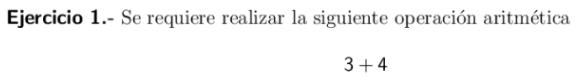
\includegraphics{e1} \\
	\begin{center}
	\textbf{Respuesta: } 0 . \\ 0 \\ dup \\ while 9 <= \\ 1 + \\ dup . \\ dup
	\end{center}
	
\item  EJERCICIO 2:\\
	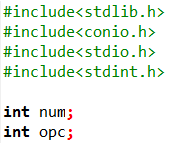
\includegraphics{e2} \\
	\begin{center}
	\textbf{Respuesta: } -9 \\ while dup \\ dup S. \\ ++ \\ 0 .
	\end{center}
	
\item  EJERCICIO 3:\\
	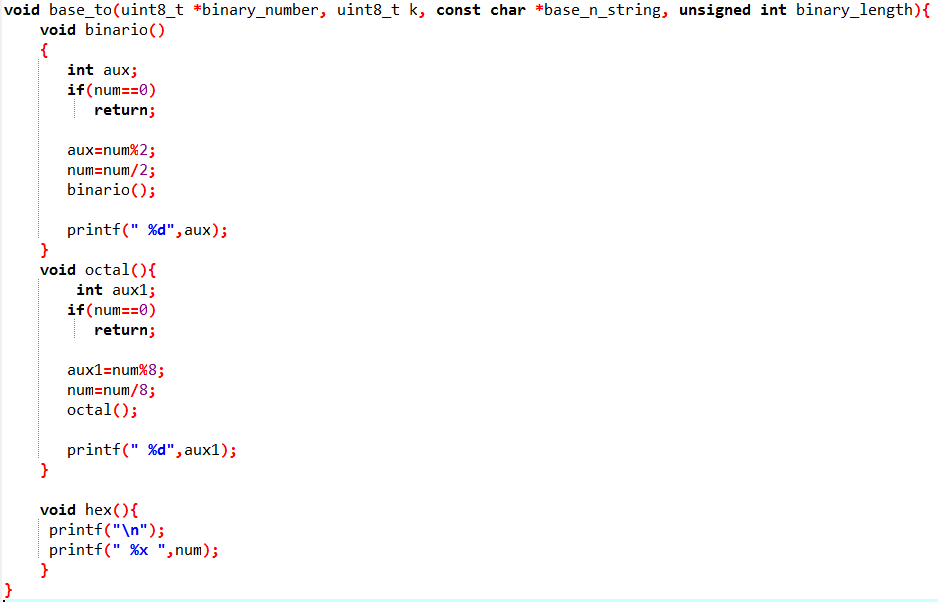
\includegraphics{e3} \\
	\begin{center}
	\textbf{Respuesta: } for 97 upto 122 \\ dup emit 
	\end{center}
\newpage
\item  EJERCICIO 4:\\
	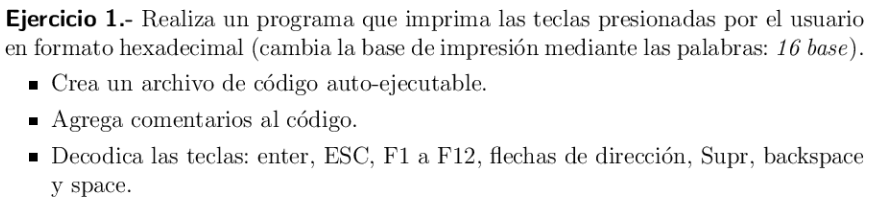
\includegraphics{e4} \\
	\begin{center}
	\textbf{Respuesta: } 65 \\ repeat \\ dup emit \\ ++ \\ dup \\ until 91 = end
	\end{center}

\end{enumerate}
\newpage
\section{Resultados (diagramas de flujo)}
\begin{enumerate}
  	\item EJERCICIO 1:\\
  	\begin{center}
	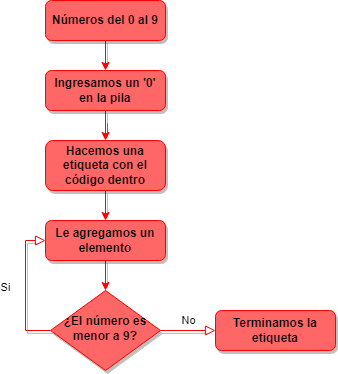
\includegraphics{diagrama1} 
	\end{center}
\newpage
	\item  EJERCICIO 2:\\
	\begin{center}
	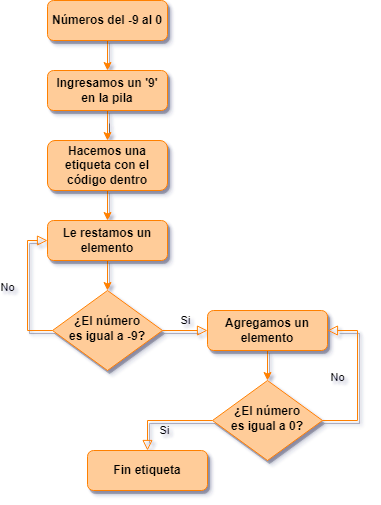
\includegraphics{diagrama2} \\
	\end{center}
\newpage	
	\item  EJERCICIO 3:\\
	\begin{center}
	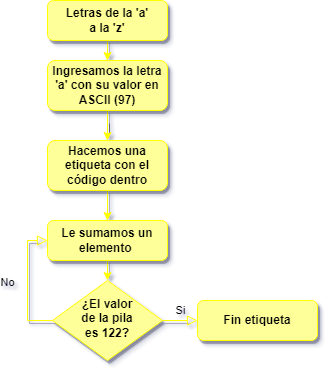
\includegraphics{diagrama3} \\
	\end{center}
\newpage	
	\item  EJERCICIO 4:\\
	\begin{center}
	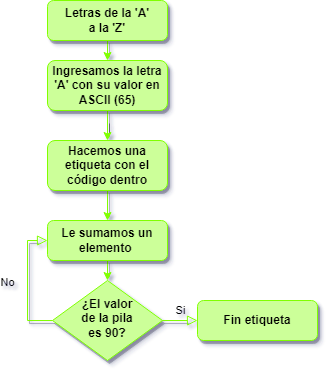
\includegraphics{diagrama4} \\
	\end{center}

\end{enumerate}

\section{Conclusiones}  
En conclusión de esta tarea puedo decir que estos ejercicio fáciles aunque ya va subiendo su complejidad no estan tan complicados ya que con conocimientos que ya tenia pude realizarlos. Pero es bueno aprender un lenguaje nuevo ya que yo ni si quiera había utilizado Linux ni mucho menos Latex, así que es una buena experiencia.

\section*{Agradecimientos}
Quiero hacer agradecimiento a mi profesor por explicarme cuando tenia dudas sobre cómo hacer los ejercicios, a mis compañeros porque varias veces me brindaron ayuda cuando tenia problemas y a mis padres en apoyarme cuando los necesito.

\begin{thebibliography}{00}
\bibitem{Alvarez2022} Becerra Alvarez, E. C. (2022, 4 octubre). ForEmb. https://drive.google.com/file/d/1Vs3F8gG-VkG6kugb4hsUSh2wFX9tYU0R/view
\end{thebibliography}

\end{document}
